\chapter{全景漫游设计评价}

全景漫游的应用场景不同于普通二维界面,其操作方式也于一般应用大相径庭,故设计评价体系也应针对一般应用相应调整。设计评价的基本形式可分为定性分分析和定量分析两种。定性分析主要用于确定事物的不易被量化的特性,带有人较强的主观思维过程。定量分析用以确认事物间某些因素或具备性质间数量上的关系,受人主观意愿影响很小,故能够较为客观地反映事物间的相对联系。

在全景漫游可视化设计中,以上两种评价方式都是十分必要的,通过定性分析可以了解到用户自身对产品的使用感受与意愿建议,而定量分析可以将交互过程拆分成独立的操作步骤、更准确地定位设计中不合适的细节所在。本章将首先介绍交互指标的涉及范围,然后细化为面向用户的评价指标用以定性分析交互的优劣性,以操作过程的量化指标分析交互形式的合理性和效率。

\section{适用于全景漫游的交互指标}
根据前文全景漫游与人的关系一章所提出的观点,全景漫游的交互质量与人的生理及心理特征均有所关联,交互指标的确定也因涵盖上述两者。全景漫游与人的生理特性间交互的质量可以体现为用户操作的便利性,如操作动作幅度是否过大、复杂任务操作的步骤是否过多、需要集中注意操作的时间是否过长等。全景漫游与人的心理特征间交互的质量可以体现为用户对交互过程的满意度,表现为用户是否可以直观地理解场景意图、是否能够自主完成预期任务、是否能够自行解决遇到的问题等。

全景漫游的交互指标以生理和心理简单划分罗列,如表\ref{tab:interaction}。

\begin{table}[htbp]
\centering
\tabcaption{全景漫游交互指标}
\vskip 5pt
\begin{tabular}{lll}
\toprule
类别 & 内容 & 参数\\
\midrule
\multirow{4}{*}{生理指标} & 视力、视野、色觉、听觉 & 视野宽度、色觉分辨力 	\\
& 触觉、温度、震动 & 温度、震动频率、频次 \\
& 肢体活动范围 & 头部活动范围 \\
& 人体舒适度、疲劳度 & 连续工作时长 \\
\midrule
\multirow{4}{*}{心理指标} & 易用性 & 操作时间、出错率 \\
& 愉悦性 & 用户满意度  \\
& 参与性 & 用户交互覆盖率  \\
& 接受性 & 用户满意率  \\
& 可靠性 & 用户满意度  \\
& 任务完成度 & 用户满意度  \\
\bottomrule
\end{tabular}
\label{tab:interaction}
\end{table}

\section{面向用户的评价指标}
面向用户的评价指标以定性评价为主,主要用于采集用户使用过程中的主观感受及反馈。为简化用户填表时的考量因素,以 1-5 级等级策略统计为标准进行问卷设计\endnote{姜强,赵蔚,王朋娇. 自适应学习系统中双向适应交互评价实证研究[J]. 现代远程教育研究,2013,(05):106-112.}。其中,1 级为非常不同意, 2 级为较不同意, 3 级为一般同意, 4 级为较同意, 5 级为非常同意。调查问卷如下表\ref{tab:questionnaire}。

\begin{table}[htp]
\centering
\tabcaption{用户使用问卷}
\vskip 5pt
\begin{tabular}{lcl}
\toprule
类别 & 序号 & 问题 \\
\midrule
\multirow{5}{*}{心理指标} & 1 & 我对该系统容易上手(\enskip) \\
& 2 & 我使用后感到愉悦(\enskip) \\
& 3 & 我有参与其中的感觉(\enskip) \\
& 4 & 我有继续使用该系统的意愿(\enskip) \\
& 5 & 我认为该系统是可靠耐用的(\enskip) \\
\midrule
\multirow{4}{*}{生理指标} & 6 & 我使用后感到疲劳(\enskip) \\
& 7 & 我使用后眼睛感到不舒服(\enskip) \\
& 8 & 我觉得头部不舒服(\enskip) \\
& 9 & 我觉得使用后很热(\enskip) \\
\bottomrule
\end{tabular}
\label{tab:questionnaire}
\end{table}

\section{操作过程的量化指标}

用户在操作全景漫游系统时也应进行记录其操作过程,得到的操作数据能够真实地体现用户在操作过程中的使用状态;对于一些不可复现或通过回忆记起的操作细节而言,通过使用记录能够更真实地反映出来。并且,在使用过程中因没有外在提示提醒,用户能够反映真实的使用习惯,也可以暴露更多的设计问题。

考虑到量化指标的特性与实际操作的可行性,量化指标的收集应注重效率,在设计验证过程中关键位置收集的若干参数好于全局收集的普遍参数。同时,在调查具有针对性的指标时也应注意指标的客观性,避免因主观原因导致的测量误差存在。

经作者整理,一些较有代表性的可测量数据如表\ref{tab:questionnaire2}。

\begin{table}[htbp]
\centering
\tabcaption{操作过程的量化指标}
\vskip 5pt
\begin{tabular}{lll}
\toprule
序号 & 问题 & 数据 \\
\midrule
1 & 用户初次打开页面至进入第一个场景的时间 & 	\\
2 &  用户在第一个场景中停留的时间 & \\
3 & 用户第一次学会使用视线停留触发物件效果的时间 & \\
4 & 用户触发全局导航栏内任一功能时间 & \\
5 & 用户是否分享、分享到何处 & \\
6 & 用户是否第二次打开应用、相隔时间 & \\
7 & 用户有无打开多个应用或场景、个数 & \\
\bottomrule
\end{tabular}
\label{tab:questionnaire2}
\end{table}

针对上述数据,第 1 项为用户完成一个有效导航操作的所用时间,可以反映导航功能的完善程度,侧面体现应用的易用性;第 2 项用户停留时间,能够反映用户的舒适度;第 3 项学习所用的时间可以反映系统中交互操作的易学程度;第 4 项导航功能可以反映用户对场景的参与度;第 5 项分享功能能够反映用户对应用的接受度和愉悦感;第 6、7 项是否再次使用可以反映用户对应用的接受度。

根据全景漫游应用的类别,上述指标可相应调整或增删。基本原则是测量用户真实的使用过程数据,以求反映交互设计的完成度和功能完整性。


\section{交互评价示例}

本评价示例以全景漫游系统至全景场景的漫游过程为用户实验过程,通过程序设计中添加统计代码的形式获得第一手用户数据,同时通过问卷形式调查用户使用体验。本例调查以自愿形式抽取了容量为 20 人的样本。实验设备照片如图\ref{fig:photo1},实验过程照片如图\ref{fig:photo2}。


\begin{figure}[htp]
\centering
\fbox{
  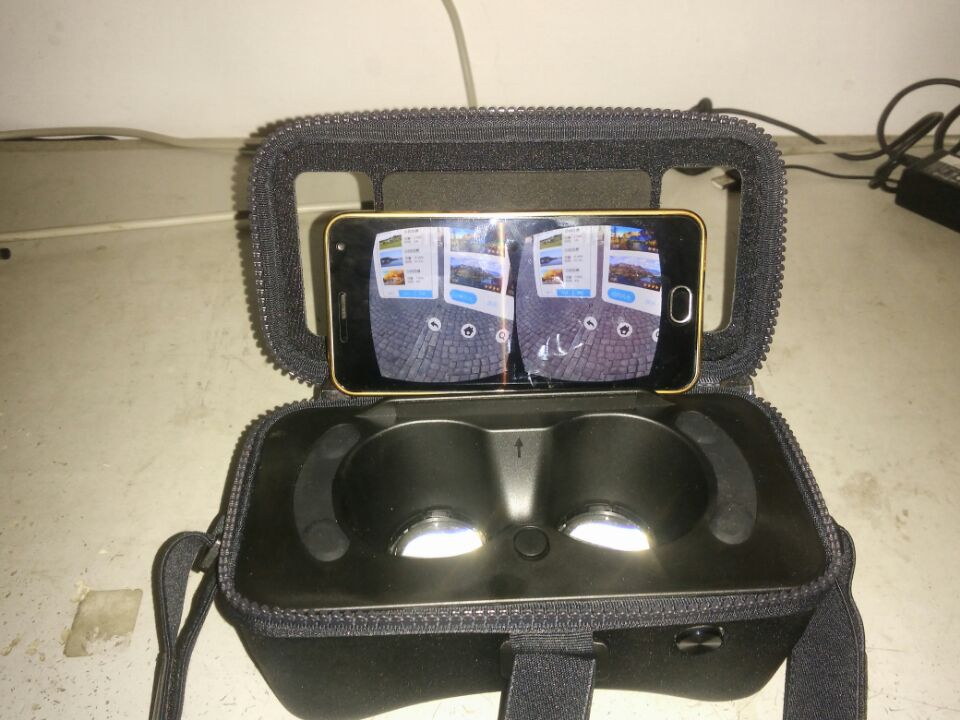
\includegraphics[width=.3\textwidth]{lab1}
}
\fbox{
  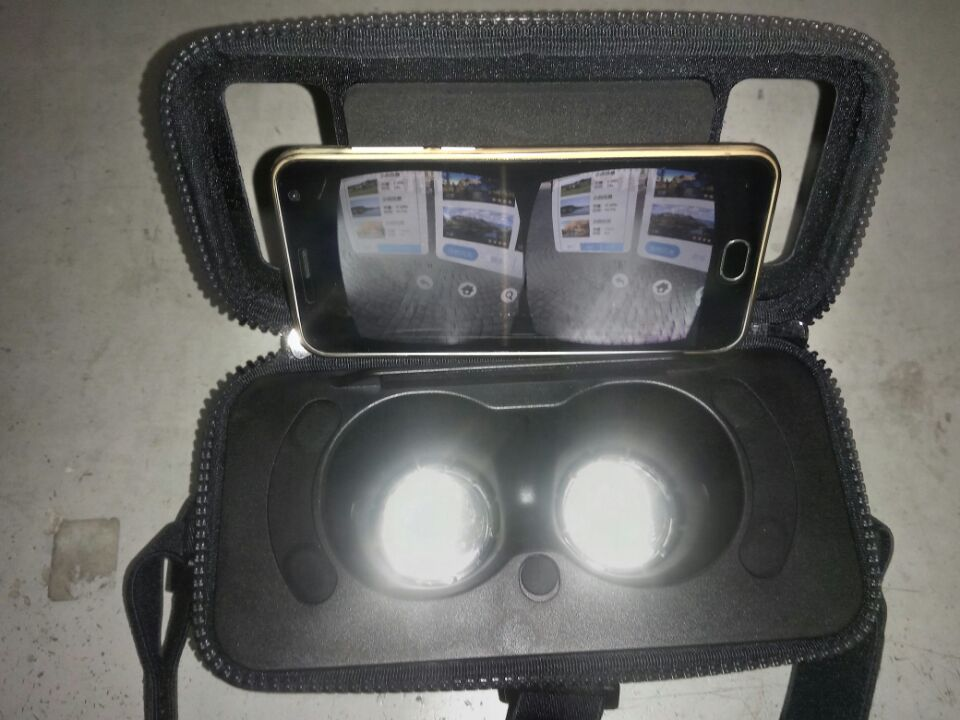
\includegraphics[width=.3\textwidth]{lab2}
}
\fbox{
  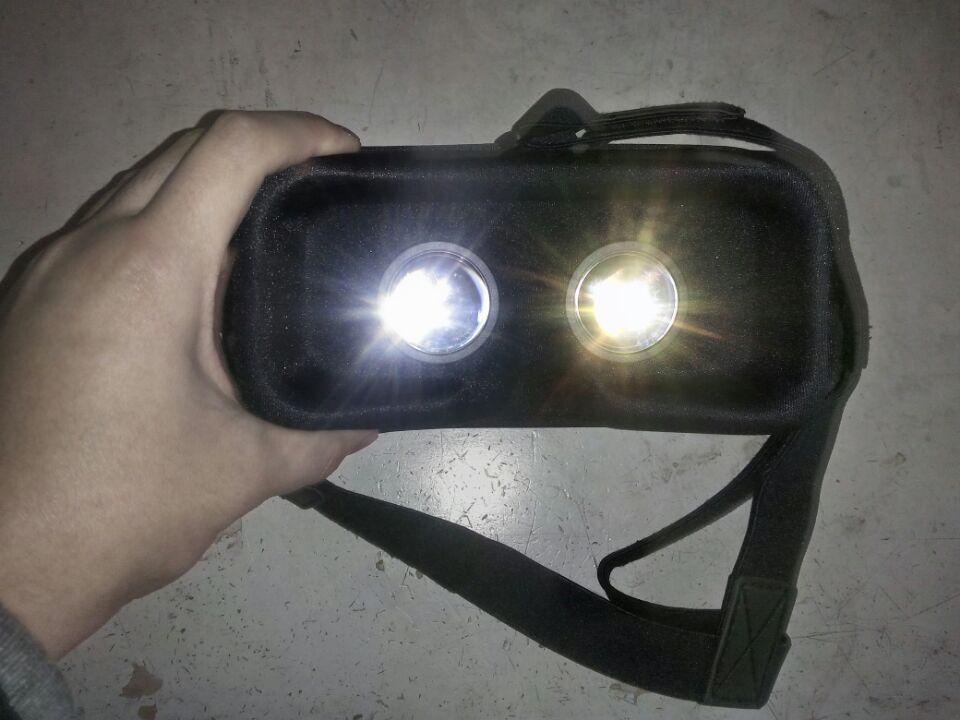
\includegraphics[width=.3\textwidth]{lab3}
}
\caption{用户实验设备照片}
\label{fig:photo1}
\end{figure}


\begin{figure}[htp]
\centering
\fbox{
  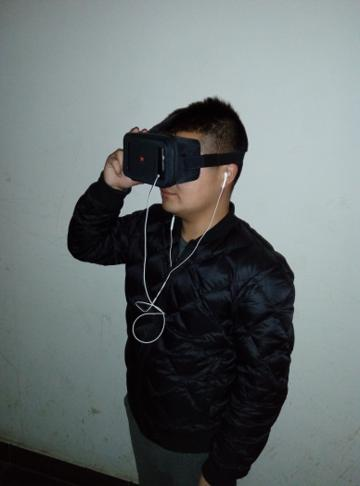
\includegraphics[width=.3\textwidth]{p1}
}
\fbox{
  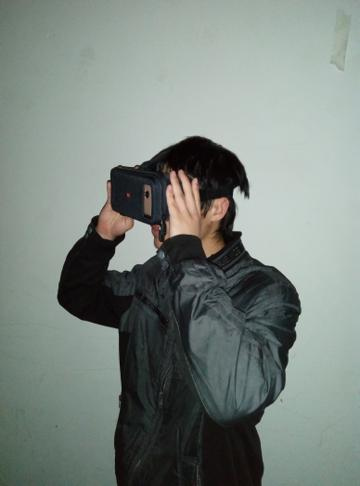
\includegraphics[width=.3\textwidth]{p2}
}
\caption{用户实验过程照片}
\label{fig:photo2}
\end{figure}


\begin{table}[ht]
\centering
\tabcaption{用户问卷数据}
\vskip 5pt
\begin{tabular}{lcllllll}
\toprule
类别 & 序号 & 问题 
& \tabincell{c}{非常\\不同意} & \tabincell{c}{较不\\同意} & \tabincell{c}{一般\\同意} & \tabincell{c}{较同意} & \tabincell{c}{非常\\同意} \\
\midrule
\multirow{5}{*}{\tabincell{c}{心理\\指标}} & 1 & 我对该系统容易上手
& 0 & 1 & 12 & 5 & 2 \\
& 2 & 我使用后感到愉悦
& 0 & 0 & 14 & 3 & 3 \\
& 3 & 我有参与其中的感觉
& 6 & 2 & 2 & 7 & 9 \\
& 4 & 我有继续使用该系统的意愿
& 0 & 1 & 11 & 3 & 5 \\
& 5 & 我认为该系统是可靠耐用的
& 5 & 2 & 8 & 4 & 1 \\
\midrule
\multirow{4}{*}{\tabincell{c}{生理\\指标}} & 6 & 我使用后感到疲劳
& 2 & 3 & 6 & 5 & 4 \\
& 7 & 我使用后眼睛感到不舒服
& 0 & 2 & 6 & 8 & 4 \\
& 8 & 我觉得头部不舒服
& 1 & 0 & 3 & 9 & 7 \\
& 9 & 我觉得使用后很热
& 0 & 0 & 7 & 9 & 4 \\
\bottomrule
\end{tabular}
\label{tab:result}
\end{table}

\begin{table}[ht]
\centering
\tabcaption{用户操作实验量化数据}
\vskip 5pt
\begin{tabular}{lll}
\toprule
序号 & 问题 & 时长/个数 \\
\midrule
1 & 用户初次打开页面至进入第一个场景的时间 & 32.2 秒	\\
2 &  用户在第一个场景中停留的时间 & 57.3 秒 \\
3 & 用户第一次学会使用视线停留触发物件效果的时间 & 8.7 秒 \\
4 & 用户触发全局导航栏内任一功能时间 & 14.1 秒 \\
5 & 用户有无打开多个应用或场景、个数 & 1.3 个 \\
\bottomrule
\end{tabular}
\label{tab:questiondata}
\end{table}

数据显示,多数用户对全景漫游的体验表示满意,但认为使用该系统存在多项生理上的不适应,该系统的可靠性和参与度仍不太高,但考虑到示例程序的简单性,参与度低是预料中的。用户操作过程基本顺利,但也有一部分用户需要经过指导后才学会使用凝视操作触发按钮等操作,可见无按键的交互形式可接受程度较低;用户在导航界面停留过程是较长的,但在场景中停留时间却没有达到 1 分钟的预期,可见场景内容的复杂度和深度尚未达到用户沉浸的标准。用户后续继续使用全景漫游的意愿不够强烈,大部分用户在 2 分钟前后就结束了全景漫游的过程,结合问卷中“感受到很热体验”的用户数量可以认识到全景漫游因其使用特殊性,易造成用户因刺激过大造成心理和生理的双重不适感受,故全景漫游设备的配戴形式仍需要改进以减轻长期使用的不适感。

总体而言,全景漫游中可视化交互设计理论的应用是符合设计预期的,用户经过一定的指导和提示后均能自主完成全景漫游的体验,这与良好的交互设计是密不可分的,同时也是因为全景漫游这种形式符合人本身的内隐性知识和日常惯例,操作方式能够很快被人理解。场景中指向标识的设置、位移控件、全局导航栏的设置等均对用户全景漫游过程产生了积极的影响,但不足的是场景应用的单一性令用户很难全面沉浸入场景,易感到疲劳,这一点或许与全景漫游没有实现视野的深度信息造成用户视觉特征信息的失调有关。